\chapter{大尺度脑电研究的谱异质同构质量指标}

\section{引言}
发展集成的脑电数据处理分析流水线平台的一个挑战是最初的预处理阶段,这一阶段需要去掉脑电伪差但也有可能去除与大脑活动有关的脑电信号。 存在脑电预处理流水线平台包括: Prep\citing{Bigdely-Shamlo et al. 2015}、Automagic\citing{Pedroni et al. 2019}、HAPPE\citing{Gabard-Durnam et al. 2018}、Lossless\citing{James et al. 2017}和Autoreject\citing{Jas et al. 2017}等等。 这些都依赖于要信号的质量指标,根据该指标可以一导联信号或者一段信号去除伪差或者进行矫正。 脑电信号要经过滤波和独立成分分析基于的伪差成分去除。 当评估脑电预处理流水线时,我们遇到多通道$\log$谱相互平行的问题,即如图\ref{Fig 1(A)}所示每个电极上所有谱是相互平行的。 这意味着头表的谱地形图在不同频率之间非常相似,意味着神经源空间对所有频率存在着在相近位置上活动的偶极子,脑电的实际源可能因为去除过多的伪差而难以识别,违背了不同频率下不同神经源共振模式的事实\citing{Hacker et al. 2017}。 在本章中,我们提出一种质量指标,能够评估脑电频谱有多大程度上在电极之间是相互平行的。

\section{研究背景}
神经电生理大数据的出现需要相应的批量自动化处理程序\citing{Bigdely-Shamlo et al., 2015}。 这些程序的例子是自动化的伪差去除\citing{Jas et al., 2017},自动的正演模型求解\citing{Huang et al., 2019; Vorwerk et al., 2018},自动的溯源分析\citing{Niso et al., 2019; Weinstein et al., n.d.}以及统计分析。 最重要的工作是对这些自动化的程序进行质量控制(quality control, QC),能够代替人脑劳动对自动化处理程序进行监督\citing{Jas et al., 2018}。 利用如脑电等电生理技术手段高的时间分辨率和频谱分析技术,人们希望刻画到神经源连接的空间模式,它可以作为脑认知功能和精神紊乱的潜在生物标记物\citing{Friston, 2011; Jirsa and McIntosh, 2007; Mars et al., 2018; Schoffelen and Gross, 2009}。 自动化数据分析的第一步是筛选脑电脑磁数据、去除伪差等等。 然后更通常的是,我们对时域的波形进行谱估计输出交叉谱,交叉谱能够代表大脑活动的全部动力学信息\citing{Nolte et al., 2019; Siegel et al., 2012} 。 最后,一种溯源分析方法能够转换头表空间的交叉谱到神经源空间\citing{Bosch-Bayard et al., 2001}。 尽管已经存在一些自动的脑电脑磁数据预处理程序,例如Automagic\citing{Pedroni et al., 2019}、autoreject\citing{Jas et al., 2017}、PREP\citing{Bigdely-Shamlo et al., 2015}、HAPPE\citing{Gabard-Durnam et al., 2018}、APP\citing{da Cruz et al., 2018}和加拿大布鲁克大学心理学院研究的lossless,尚没有一个能够检查伪差去除后的频域失真。 尽管在实际中我们难以知道脑电脑磁数据无噪声信号的集标准,但可以认为应用越多越复杂的伪差去除程序,也有可能去除与脑活动相关的信号。 在结合强力的算法进行伪差去除后得到的脑电脑磁好看的波形可能离大脑活动的内在动力学相差较远或者改变了大脑的源活动的连接空间模式。

然而,电生理神经成像将无创地记录到的脑电脑磁数据视为大脑活动信号,大脑信号的微弱和传感器的敏感更容易在得到的脑电磁记录中混有各种各样的噪声,采集的数据数据常不是很好看。 无论脑电脑磁数据经过了怎样的预处理,在进一步分析动力学或者源活动之前的必要一步是对头表上估计得到的频谱进行质量分析。 我们发现$\log$转换之后的频谱在所有电极之间是相互平行的,即Parallel LOg Spectra (PaLOS) 问题。 如图\ref{fig1}所示,较短频率间隔上的谱地形图呈现稳定相似的空间模式,这可能表明神经源偶极子的震荡情况是基本不变的,与大脑具有依赖于频域高度震荡的动力学信息这一认识相背离\citing{Cabral et al., 2017; Deco et al., 2011}。 也有研究认为大脑连接更可能依赖于频率呈现不同的模式而不是静态固定的\citing{Chang and Glover, 2010; Foster et al., 2015; Hacker et al., 2017; Thompson and Fransson, 2015}。

在本章中,我们提出用第一个共同的主要成分\citing{Trendafilov, 2010}在交叉谱数据中所有频率上占的比例作为判定伪差去除后的脑电脑磁数据是否具有PaLOS现象的质量准则。 直观地推理,如果多通道功率谱在所有频率上电极之间是相互平行的,所有通道的谱曲线就是一个共同的主要尺度加减不同尺度平移后的结果。 多通道功率谱相互平行这个单变量的问题可以推广到交叉谱的多变量的情况, 所有频率的交叉谱由共同主要交叉谱空间模式的尺度变换版本合成且其中一个具有解释全部方差的最大成份。


为了验证第一个共同的主要成分是合适的质量准则,我们需要考虑一些可能人为地通过插值增加通道之间相关性共线性而引入的PaLOS问题,例如脑电的参考过程\citing{Hu et al., 2018},使用独立成分分析的去除过多的成分,插值修复坏道,和眼电的回归等等。 

\section{研究方法}
\subsection{模型}
%In magnetic-electrical recordings spectrum analysis, the recordings are segmented, and each segment is
%taken the discrete Fourier transform. If y is the Fourier coefficient at the frequency  of the data at
%segment s ( 1,...,n  = and 1,..., s s = n ), z is a 1 k n  vector of ones, indicating the linearly additional
%effect of k n components, and  b is a 1 k n  vector, consisting of the Fourier coefficients of k n
%components at frequency  and epoch s , ( , )
%%k
%%C
%%n N   b 0 Σ , diag( )   Σ = σ , 1 [ ,..., nk ]
%%   =   T

\subsection{特征}
\subsection{影响因素}

\section{结果}
The PaLOS index was applied to 1525 eyes-closed resting EEGs from healthy controls: 1224 CMI-HBN cases with
the Hydro GSN129 headset, 250 Cuba CHBMP EEGs with the 10-10 64chn headset, and 51 Barbados EEGs with
10-20 19chn headset. The 1224 EEGs include the raw data with redundant artifacts and finally clean data by
Automagic. The Cuba and Barbados EEGs contain the raw data with very minor artifacts and only the stationary
epochs picked by the neurophysiologists. The median of PaLOS index for the cleaned CMI EEG decreased to 0.66
<< 0.98 of that for the noisy raw data; the PaLOS index of Cuba and Barbados raw EEGs without EOG but with
very minor artifacts were 0.3-0.5, while that of the clean stationary signals were a little bit increased (See Fig.
1(C)). This demonstrated that PaLOS index can indicate the homogeneity in the spectral profile and the
multichannel time series.
\begin{figure}[!ht]
	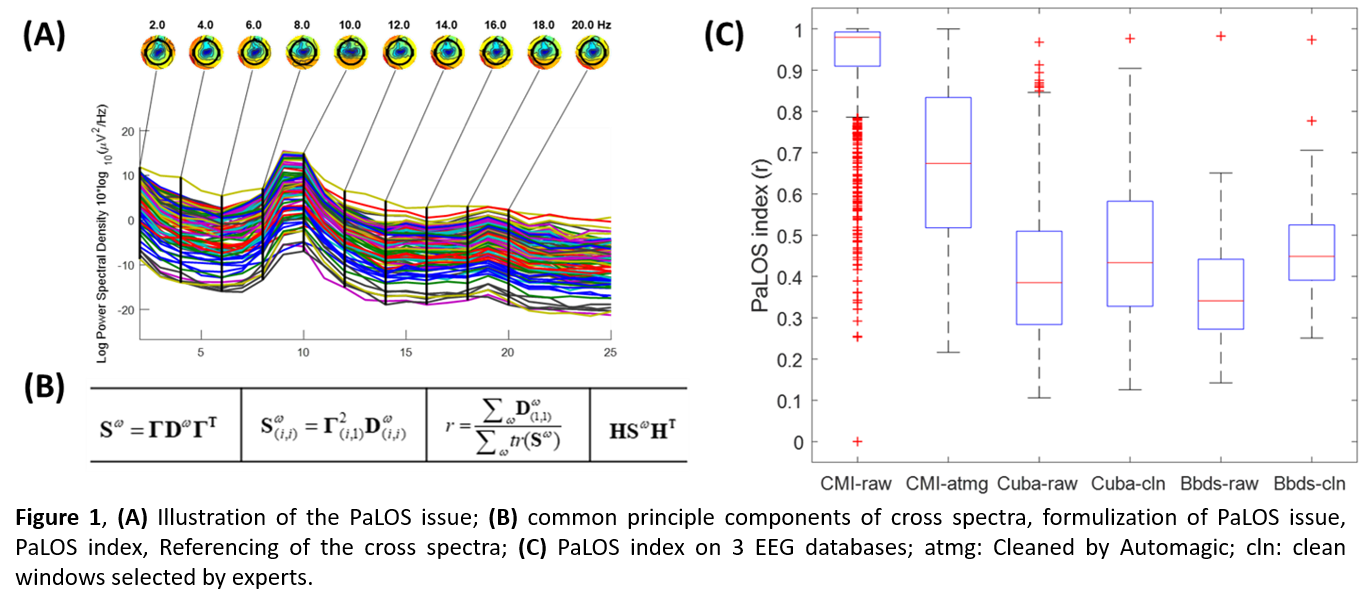
\includegraphics[width=15cm]{pic/palos/figure1.png}
	\caption{}
	\label{fig1}
\end{figure}
In addition, the PaLOS index was applied to each step of Automagic and the referencing. The quality of randomly
picked 10 CMI cases were Bad (349, 904), Ok (117, 948), and Good for the rest at the final step. 10 cases showed
that mostly Prep, Reg and MARA increased the PaLOS index, while Filt reduced that (See Fig. 2(A)). The bad cases
(349, 904) showed different stepwise changing of PaLOS index from the others, and the final PaLOS index were
higher. The Fig. 2(B) displayed the spectra curves and topographies for a Good 112 and a bad 349. The PaLOS
index are 0.38-0.56 for unparalleled 112 and 0.86-0.97 for parallel 349. Regarding the reference, the AR and
REST derived more supportive PaLOS indexes (0.39<0.55, 0.97>0.86) for Good and Bad than the Rb.
\begin{figure}[!ht]
	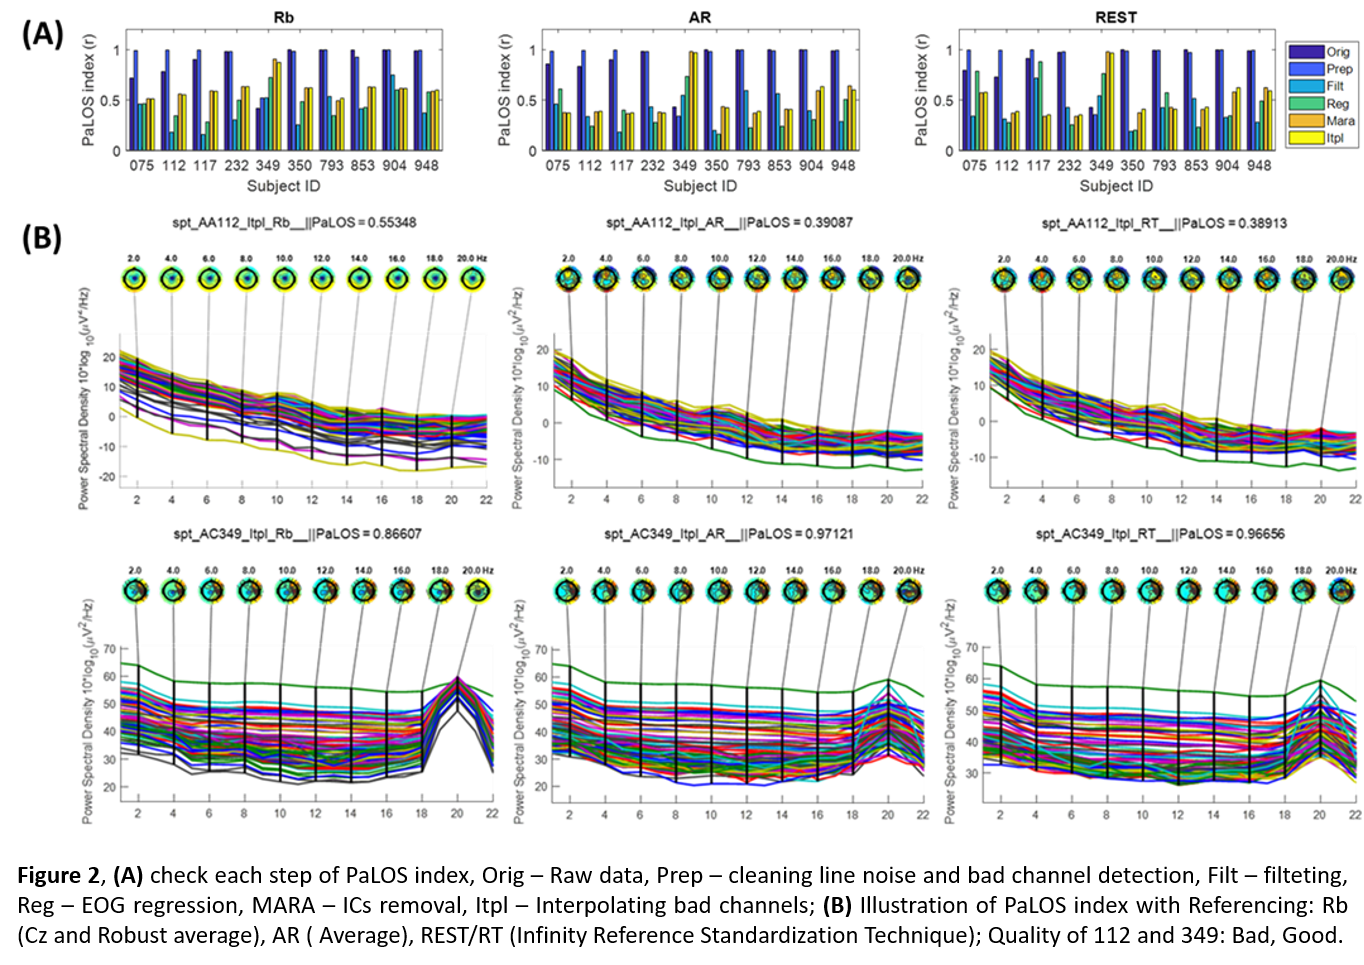
\includegraphics[width=15cm]{pic/palos/figure2.png}
	\caption{}
	\label{fig2}
\end{figure}
\section{本章小结}
PaLOS index can be a promising metric of checking the homogeneity of the spectra profile and the extent of
artifacts rejection in the mega EEG cleaning pipeline.